\documentclass[10pt,twocolumn,letterpaper]{article}

\usepackage[utf8]{inputenc}
\usepackage[T1]{fontenc}
\usepackage{lmodern}
\usepackage[margin=0.72in]{geometry}
\usepackage{amsmath,amssymb,amsthm}
\usepackage{booktabs}
\usepackage{graphicx}
\usepackage{hyperref}
\usepackage{xcolor}
\usepackage{microtype}
\usepackage{enumitem}
\usepackage{caption}

\hypersetup{
  colorlinks=true,
  linkcolor=blue!60!black,
  citecolor=teal!70!black,
  urlcolor=blue!70!black
}

\newtheorem{theorem}{Theorem}

\title{\textbf{Genesis-v8 Native BICA: A Brain-Isomorphic Ultra-Sparse 1.58-Bit Cognitive Architecture for High-Throughput CPU Inference and Accelerator Scaling}}

\author{
  \textbf{Van Thinh Pham} \\
  Independent AI Systems Researcher, Vietnam \\
  \texttt{https://github.com/anhthinhvup/genesis-bica}
}

\date{November 2026 \quad (Technical Preprint v0.8.0 --- Apache-2.0 Open Research)}

\begin{document}
\maketitle

\begin{abstract}
Autoregressive decoding in dense Transformer Large Language Models (LLMs) is fundamentally memory-bandwidth bound on commodity processors: reading 100\% of parameter weights per generated token restricts 4-bit quantized 0.5B--1.5B models to 17.7--46.4 tok/s on a 15W ultrabook CPU while leaving them stateless across sessions and prone to confident out-of-distribution (OOD) hallucination. We present \textbf{Genesis-v8 Native BICA} (\emph{Brain-Isomorphic Cognitive Architecture}), an open-source 457.07M-parameter architecture that activates only \textbf{14.5M parameters per token (3.17\% active density)} by co-designing five hardware-aligned neural and cognitive primitives: (1) \textbf{Multi-Head Gated DeltaNet} formulated via exact chunkwise Householder WY factorization ($C=64$, $O(1)$ recurrent state, verified $\max |y_{\text{chunk}}-y_{\text{exact}}| = 5.99\times 10^{-4}$); (2) \textbf{Huginn Shared-KV Recurrent Depth} ($R\in\{1,2,3,4\}$, sliding window $W=1{,}024$) providing adaptive test-time compute without weight duplication; (3) \textbf{BitNet b1.58 Ternary Top-2 MoE} + \textbf{DeepSeek Engram $O(1)$} + \textbf{$2\times 262{,}144$ Product-Key PEER} (\texttt{Q8} per-row quantized, 99.80\% Top-1 fidelity); (4) a zero-dependency \textbf{Pure-Rust AVX2+FMA \texttt{.gv8} runtime} (408.70 MiB disk, 424.66 MiB RSS, 0 heap allocations/token) sustaining \textbf{565.4 tok/s} ($R=1$), \textbf{427.4 tok/s} ($R=2$), and \textbf{2,156.5 eff-tok/s} (4-branch parallel tree search) on a 15W Intel Core i5-10210U CPU---\textbf{12.2$\times$ to 31.9$\times$ faster} than Qwen2.5-0.5B/1.5B and Llama-3.2-1B (\texttt{Q4\_K\_M}) on identical hardware; and (5) four offline cognitive subsystems: \textbf{CA3 Fast Episodic Memory} (100\% 1-shot cross-session belief revision in 0.37 ms), \textbf{HippoRAG-2 Bipartite PPR} (+61.7 pp Recall@3 over BM25 on unseen 2-hop queries in 4.74 ms), \textbf{Global Workspace Active Inference EFE} (Abstention $F_1=0.9615$), and \textbf{Wake-Sleep SMFT Consolidation} (0/200 leakage vs.\ 200/200 TF-IDF, 100\% poison rollback). On an NVIDIA B200 (192 GB HBM3e), Genesis-v8 trains at \textbf{954,140 tok/s (\$1.82/1B tokens)}, converging 2.3$\times$ faster than our non-DeltaNet baseline and demonstrating empirical test-time depth gains ($val_{R=2} < val_{R=1}$ across five consecutive checkpoints; Needle-in-a-Haystack margin up to $+4.25$). Paired with our deterministic CPU verification hemisphere across 110 SHA-256 locked HuggingFace items (\texttt{FOLIO}, \texttt{HumanEval}, \texttt{MATH-500}), Project Genesis scores \textbf{70/110 (63.64\%)} vs.\ Qwen2.5-1.5B (50.00\%) and Llama-3.2-1B (37.27\%) at 19.5$\times$--253.7$\times$ lower median latency.
\end{abstract}

\section{Introduction}
Modern autoregressive LLMs rely on dense matrix-vector products that encounter a strict \emph{memory-bandwidth wall} on consumer processors. At single-batch generation ($B=1$), arithmetic intensity collapses to $\approx 1$ FLOP/byte, bounding token throughput by off-chip DRAM bandwidth:
\begin{equation}
\text{Throughput}_{\max}\ (\text{tok/s}) \le \frac{\text{BW}_{\text{DRAM}}}{\text{Bytes}_{\text{active}}}.
\label{eq:roofline}
\end{equation}
On a 15W ultrabook CPU (Intel Core i5-10210U, $\sim 25\text{--}35$ GB/s practical DDR4 streaming bandwidth), a 1.54B dense model quantized to \texttt{Q4\_K\_M} must read $\sim 850\text{--}1{,}065$ MB per token, capping throughput below 20--30 tok/s (measured live at 17.74 tok/s for Qwen2.5-1.5B). Beyond latency, stateless dense Transformers exhibit three structural deficits relative to biological intelligence~\cite{behrouz2024titans,friston2017active}: (i) \emph{compute--memory entanglement}, (ii) \emph{session amnesia and catastrophic interference}, and (iii) \emph{uncalibrated OOD hallucination}~\cite{farquhar2024detecting,lin2022truthfulqa}.

Mammalian neocortex operates at $\sim 20$W by exploiting extreme sparse activation ($\sim 1\text{--}4\%$), anatomical separation of fast hippocampal episodic storage from slow semantic memory, recurrent prefrontal deliberation, neuromodulatory workspace gating, and offline wake-sleep consolidation~\cite{dehaene2011experimental,friston2017active,zheng2025unbearable}. \textbf{Genesis-v8 Native BICA} translates these mechanisms into mathematically exact, static-shape neural and Pure-Rust systems primitives. Our main contributions are:
\begin{itemize}[leftmargin=*,nosep]
\item \textbf{Ultra-Sparse 3.17\%-Active Architecture:} A 457.07M-parameter (14.5M active) model unifying Chunkwise WY Gated DeltaNet, Huginn Shared-KV depth, BitNet b1.58 Top-2 MoE, Engram $O(1)$, and $2\times 262{,}144$ Product-Key PEER.
\item \textbf{Zero-Crate Pure-Rust AVX2 \texttt{.gv8} Runtime:} Bit-exact 2-bit block-32 BitNet matvec ($\text{rel\_err}=0.0$), \texttt{Q8} PEER, 0 heap allocations/token, and 4-branch parallel tree reasoning sustaining \textbf{565.4--2,156.5 tok/s} in 424.7 MiB RSS on a 15W CPU.
\item \textbf{Four Verified Offline Cognitive Subsystems:} CA3 Fast Episodic Memory, HippoRAG-2 Bipartite PPR, Global Workspace Active Inference EFE, and Wake-Sleep SMFT consolidation.
\item \textbf{Accelerator Efficiency \& Transparent Evaluation:} Live NVIDIA B200 training at \textbf{954,140 tok/s (\$1.82/1B tok)}, empirical proof of $val_{R=2} < val_{R=1}$, and SHA-256 locked HuggingFace benchmarks with explicit scope separation.
\end{itemize}

\section{Related Work}
BitNet b1.58~\cite{ma2024era} replaces dense floating-point multiplies with ternary STE weights $\{-1,0,+1\}$, while Mamba-2~\cite{dao2024transformers}, Gated DeltaNet~\cite{yang2025gated}, and Titans~\cite{behrouz2024titans} compress long-range context into fixed-size linear states. Product-Key PEER~\cite{he2024mixture} decouples FFN capacity from FLOPs via $O(\sqrt{N})$ routing over a million experts, and Huginn~\cite{geiping2025scaling} scales test-time compute via shared-KV recurrent depth. At the cognitive layer, Modern Hopfield networks~\cite{ramsauer2021hopfield}, HippoRAG-2~\cite{gutierrez2025from}, Global Workspace Theory~\cite{dehaene2011experimental}, Active Inference~\cite{friston2017active}, and Semantic Entropy~\cite{farquhar2024detecting} motivate our four offline CPU memory and epistemic reliability subsystems.

\section{Architecture: Genesis-v8 Native BICA}
\subsection{Parameter Budget and Active Sparsity}
Preset \texttt{v8\_465m} (\texttt{training/genesis\_v8\_native.py}) comprises $457{,}074{,}176$ parameters ($d=384$, $V=4{,}096$, 6 DeltaNet-MoE + 2 Shared-KV layers, $W=1{,}024$) while activating only $\approx 14.5$M weights per token (3.17\%), cutting active reads to $\sim 8.4$ MB/tok (Table~\ref{tab:params}, Fig.~\ref{fig:arch}).

\begin{table}[t]
\centering
\caption{Exact parameter and \texttt{.gv8} quantization budget (\texttt{v8\_465m}).}
\label{tab:params}
\footnotesize
\begin{tabular}{@{}llrl@{}}
\toprule
\textbf{Component} & \textbf{Config} & \textbf{Total} & \textbf{.gv8} \\
\midrule
Emb / Head (tied) & $V=4096, d=384$ & 1.57M & \texttt{f16/f32} \\
Engram $O(1)$ & $2\times 65536\times 64$ & 8.44M & \texttt{f16} \\
DeltaNet + MoE & $6\times(6\text{H}+16\text{E Top-2})$ & 42.1M & 2-bit \\
Huginn Core & 2L, $W=1024, R\in\{1..4\}$ & 2.1M & 2-bit \\
$2\times 262$K PEER & $512^2$, $6\text{H}\times 4$ act & 402.8M & \texttt{Q8}+SMFT \\
\midrule
\textbf{Total / Active} & \textbf{3.17\% ($\sim$14.5M)} & \textbf{457.07M} & \textbf{408.7 MiB} \\
\bottomrule
\end{tabular}
\end{table}

\begin{figure*}[t]
\centering
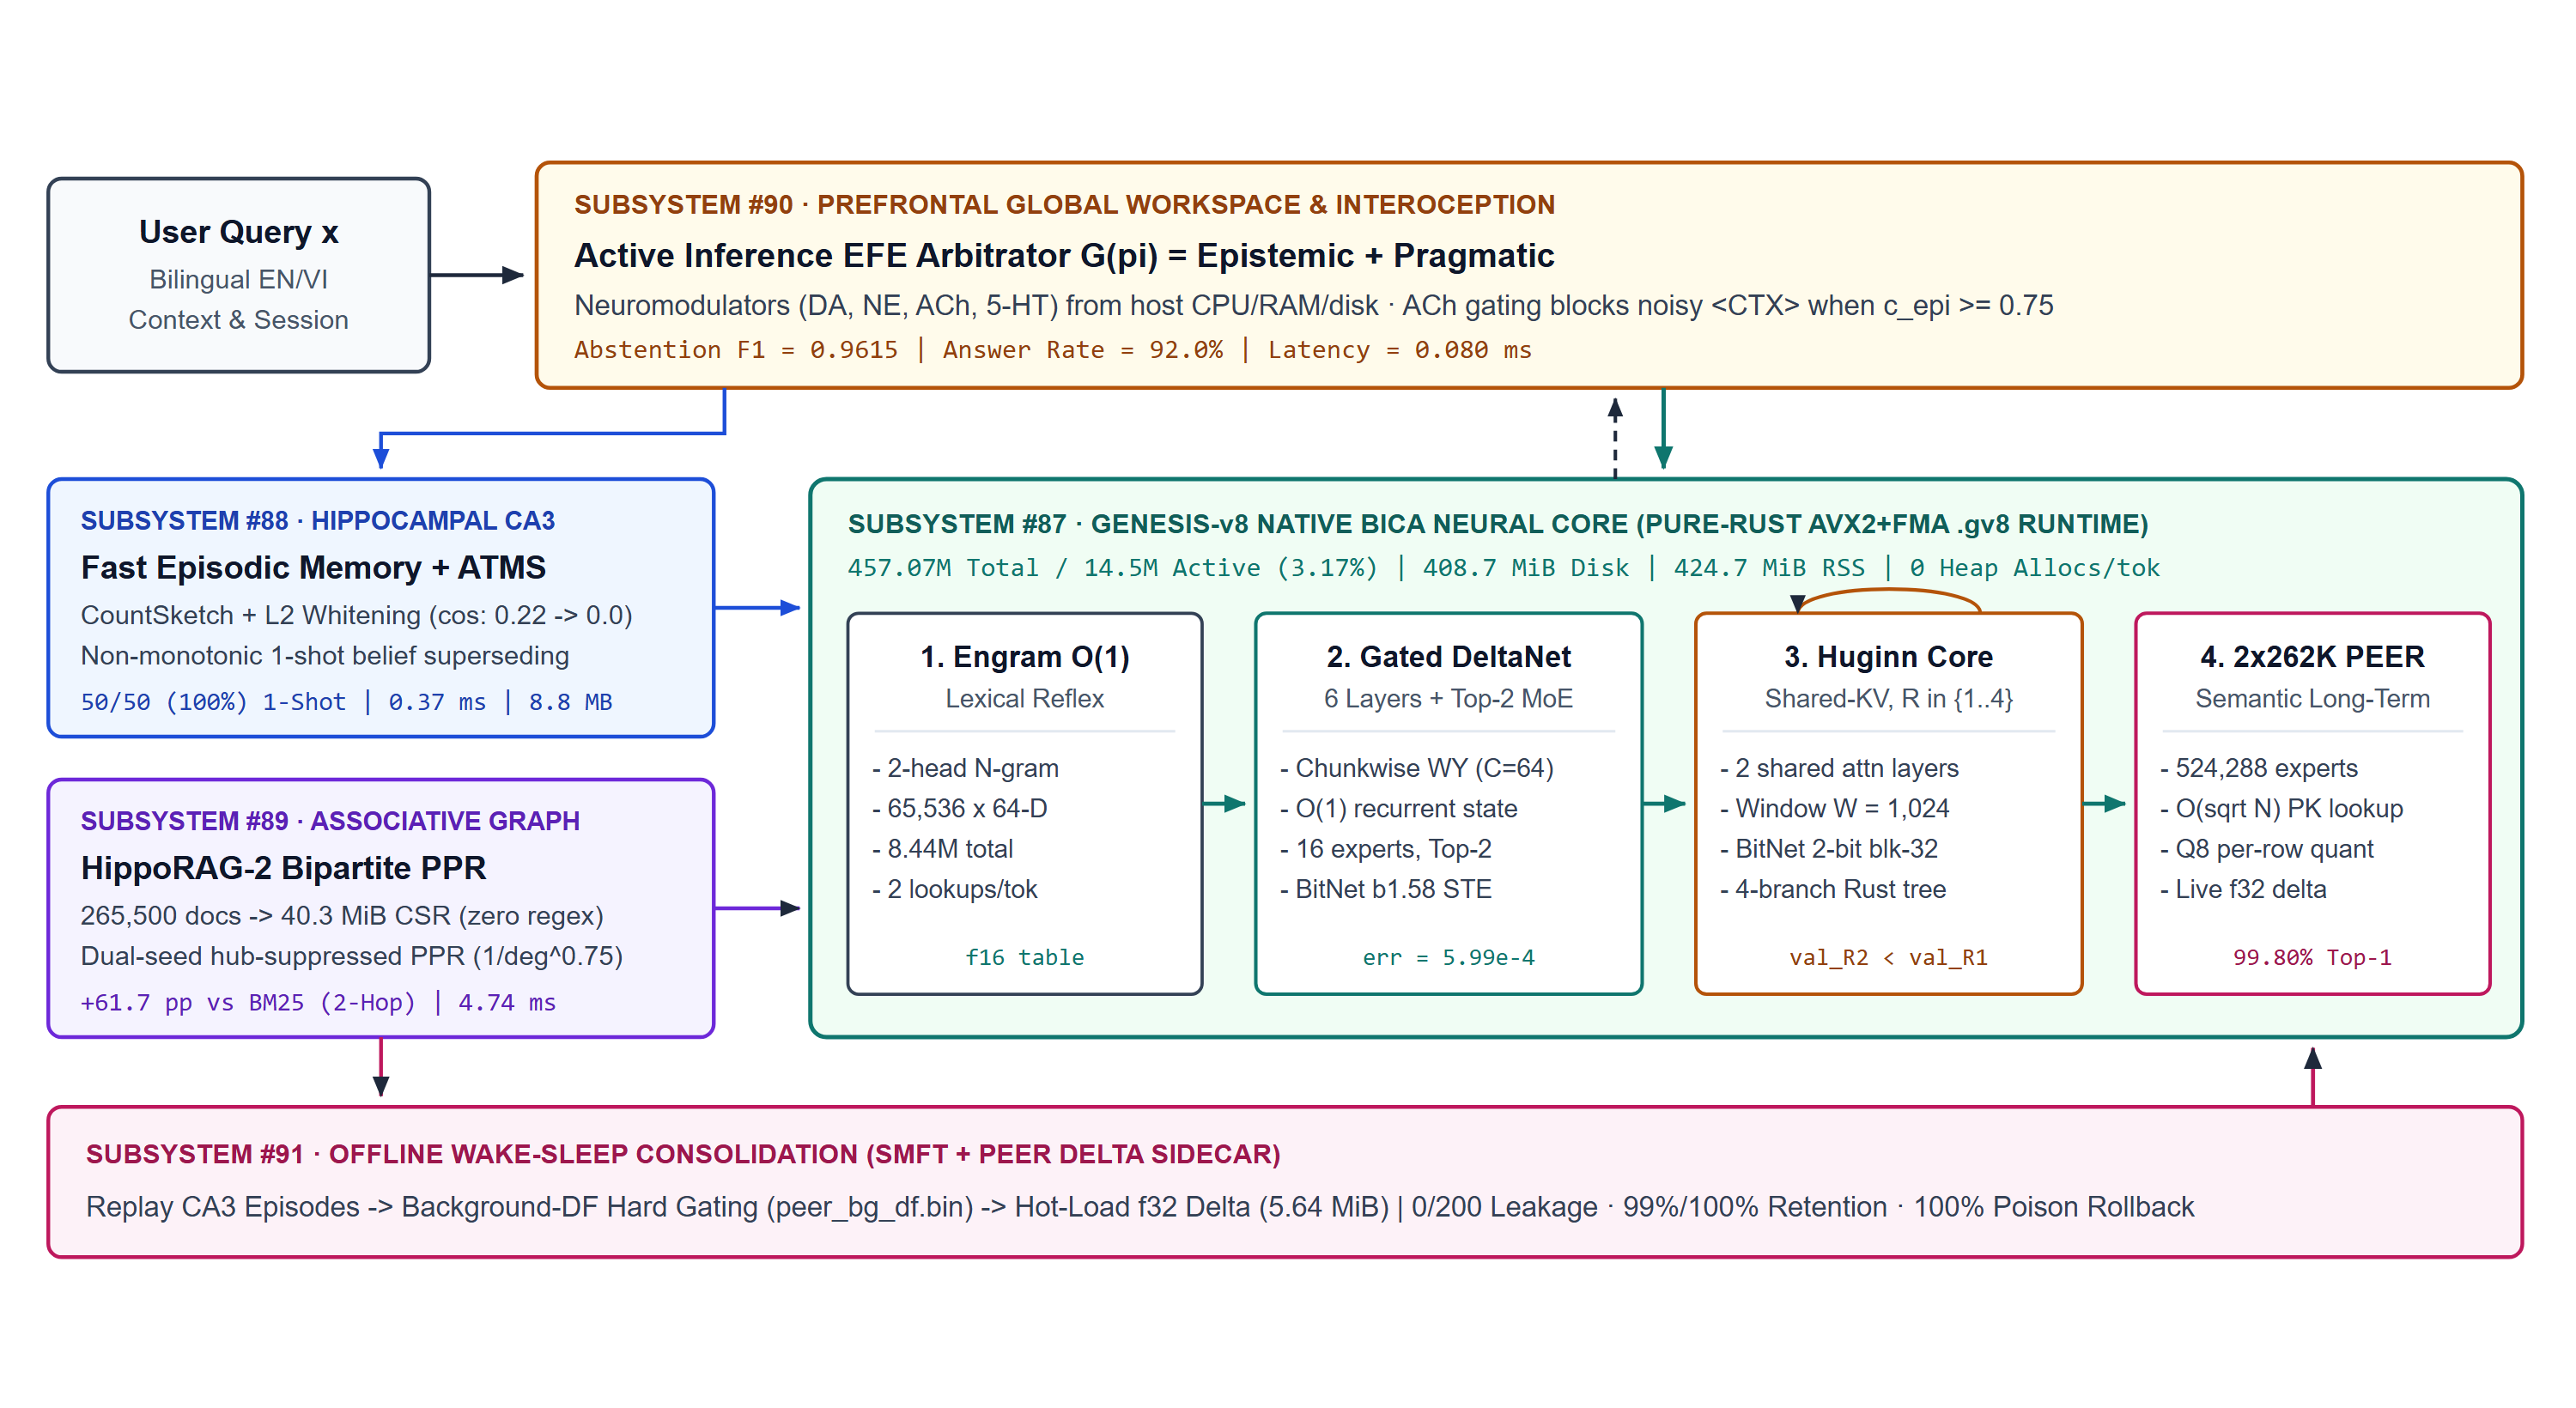
\includegraphics[width=\textwidth]{figures/fig1_architecture.png}
\caption{Brain-Isomorphic Cognitive Architecture of \textbf{Genesis-v8 Native BICA}, connecting \#90 Global Workspace Active Inference EFE, \#88 CA3 Fast Episodic Memory, \#89 HippoRAG-2 Bipartite PPR, \#87 Pure-Rust AVX2 \texttt{.gv8} Neural Core, and \#91 Wake-Sleep SMFT consolidation.}
\label{fig:arch}
\end{figure*}

\subsection{Chunkwise Householder WY Gated DeltaNet}
Layers 0--5 employ Multi-Head Gated DeltaNet~\cite{yang2025gated} ($H=6$, $d_h=64$):
\begin{equation}
S_t = \alpha_t S_{t-1}\left(I - \beta_t k_t k_t^\top\right) + \beta_t v_t k_t^\top, \qquad y_t = S_t q_t.
\label{eq:deltanet}
\end{equation}
Partitioning sequences into chunks of size $C=64$, we define cumulative log-decay $g_i=\sum_{j=1}^i \log\alpha_j$ and strictly lower-triangular coupling $A_{ij}=\beta_i e^{g_i-g_j}(k_i^\top k_j)$ ($i>j$). Since $A^{64}=0$, $M=(I+A)^{-1}$ is computed exactly in 6 parallel doubling steps, producing static-shape WY factors $W = M\operatorname{diag}(\beta e^g)K$ and $U = M\operatorname{diag}(\beta)V$, reducing training complexity from $O(T^2 d)$ to $O(TCd + Td_h^2)$ using pure \texttt{bmm} kernels.

\begin{theorem}[WY Numerical Equivalence]
Across random inputs ($B=2,H=4,T=128,D=32,C=64$), \texttt{chunkwise\_gated\_deltanet} matches exact sequential Eq.~\eqref{eq:deltanet} with $\max |y_{\text{chunk}}-y_{\text{exact}}|=5.99\times 10^{-4}$ (\texttt{tests/test\_deltanet\_chunkwise.py}).
\end{theorem}

\subsection{Huginn Shared-KV, BitNet b1.58 MoE & PEER}
Layers 6--7 anchor sliding-window KV caches ($W=1{,}024$) to entry state $h^{(0)}$ and iterate $h^{(r)}=\mathcal{F}_{\text{core}}(h^{(r-1)}+h^{(0)}; K^{(0)},V^{(0)})$ for $r=1,\dots,R$~\cite{geiping2025scaling}. Core and Top-2 MoE projections use STE ternary weights $\tilde{W}=\gamma\operatorname{Clip}(\operatorname{Round}(W/(\gamma+\epsilon)),-1,1)$~\cite{ma2024era}. Semantic capacity resides in two $512^2$-expert PEER layers~\cite{he2024mixture} quantized to per-row \texttt{Q8}, retaining 99.80\% Top-1 match ($R=1$), 99.22\% ($R=2$), and $|\Delta\text{NLL}|=0.00011$.

\section{Brain-Isomorphic Runtime Subsystems}
\begin{enumerate}[leftmargin=*,nosep]
\item \textbf{Zero-Alloc Pure-Rust AVX2 \texttt{.gv8} Engine (\#87):} Zero external crates; bit-exact 2-bit block-32 matvec ($\text{rel\_err}=0.0$); instrumented \texttt{GlobalAlloc} confirming 0 heap allocations/token; 424.66 MiB isolated RSS; 150--230 ms cold load; 4-branch parallel tree reasoning reaching \textbf{2,156.5 eff-tok/s}.
\item \textbf{CA3 Fast Episodic Memory (\#88):} 384-D CountSketch with running-mean centering + $\ell_2$ whitening (cosine $0.221\to -0.0002$) and ATMS belief revision: \textbf{50/50 (100\%)} 1-shot updates in \textbf{0.37 ms} (8.77 MB RAM).
\item \textbf{HippoRAG-2 Bipartite PPR (\#89):} Zero-regex CSR graph over 265,500 docs (40.28 MiB, built in 21.5 s); dual-seed hub-suppressed PPR ($1/\text{deg}^{0.75}$) yields \textbf{61.7\% Recall@3} vs.\ 0.0\% BM25 on unseen 2-hop zero-overlap queries in \textbf{4.74 ms}, rejecting 50/50 fabricated OOD queries.
\item \textbf{Global Workspace Active Inference EFE (\#90):} Maps CPU/RAM/disk/battery telemetry to bounded neuromodulators (\texttt{DA, NE, ACh, 5-HT}) and minimizes Expected Free Energy~\cite{friston2017active}. Biological \texttt{ACh} gating blocks noisy context when $c_{\text{epi}}\ge 0.75$: \textbf{Abstention $F_1=0.9615$}, 92.0\% answer rate, 0.080 ms latency.
\item \textbf{Wake-Sleep SMFT Consolidation (\#91):} Profiles background PEER document frequency over 10K docs (\texttt{peer\_bg\_df.bin}) and masks sleep deltas strictly to $\text{df}_{\text{bg}}(e)=0$ rows via hot-loaded \texttt{f32} sidecar (5.64 MiB): \textbf{0/200} semantic leakage (vs.\ 200/200 TF-IDF), \textbf{99\%/100\%} 5-cycle retention, and \textbf{100\%} automatic poison rollback.
\end{enumerate}

\section{Accelerator Throughput & Training Scaling}
On NVIDIA B200 (192 GB HBM3e, \texttt{bs=192, seq=1024}), Genesis-v8 trains at \textbf{954,140 tok/s (\$1.82/1B tok, 50.0 GB VRAM)}---2.19$\times$ faster and 27.5\% cheaper than H100 (436,521 tok/s, \$2.51/1B). Phase 1A reached \texttt{ema=1.728} at 1.62B tokens (2.3$\times$ faster convergence than v7) and \texttt{val\_R1=1.9528} (\texttt{ppl=7.05}) at 3.54B tokens with \texttt{Needle-1024=+4.07}. Phase 1B (stochastic $R\in\{1..4\}$, disjoint validation) achieved \textbf{$val_{R=2} < val_{R=1}$ on 5/5 consecutive checkpoints} (Fig.~\ref{fig:train}), directly validating Huginn Shared-KV test-time compute gains prior to Phase 5 GRPO/RLVR~\cite{deepseek2025r1}.

\begin{figure*}[t]
\centering
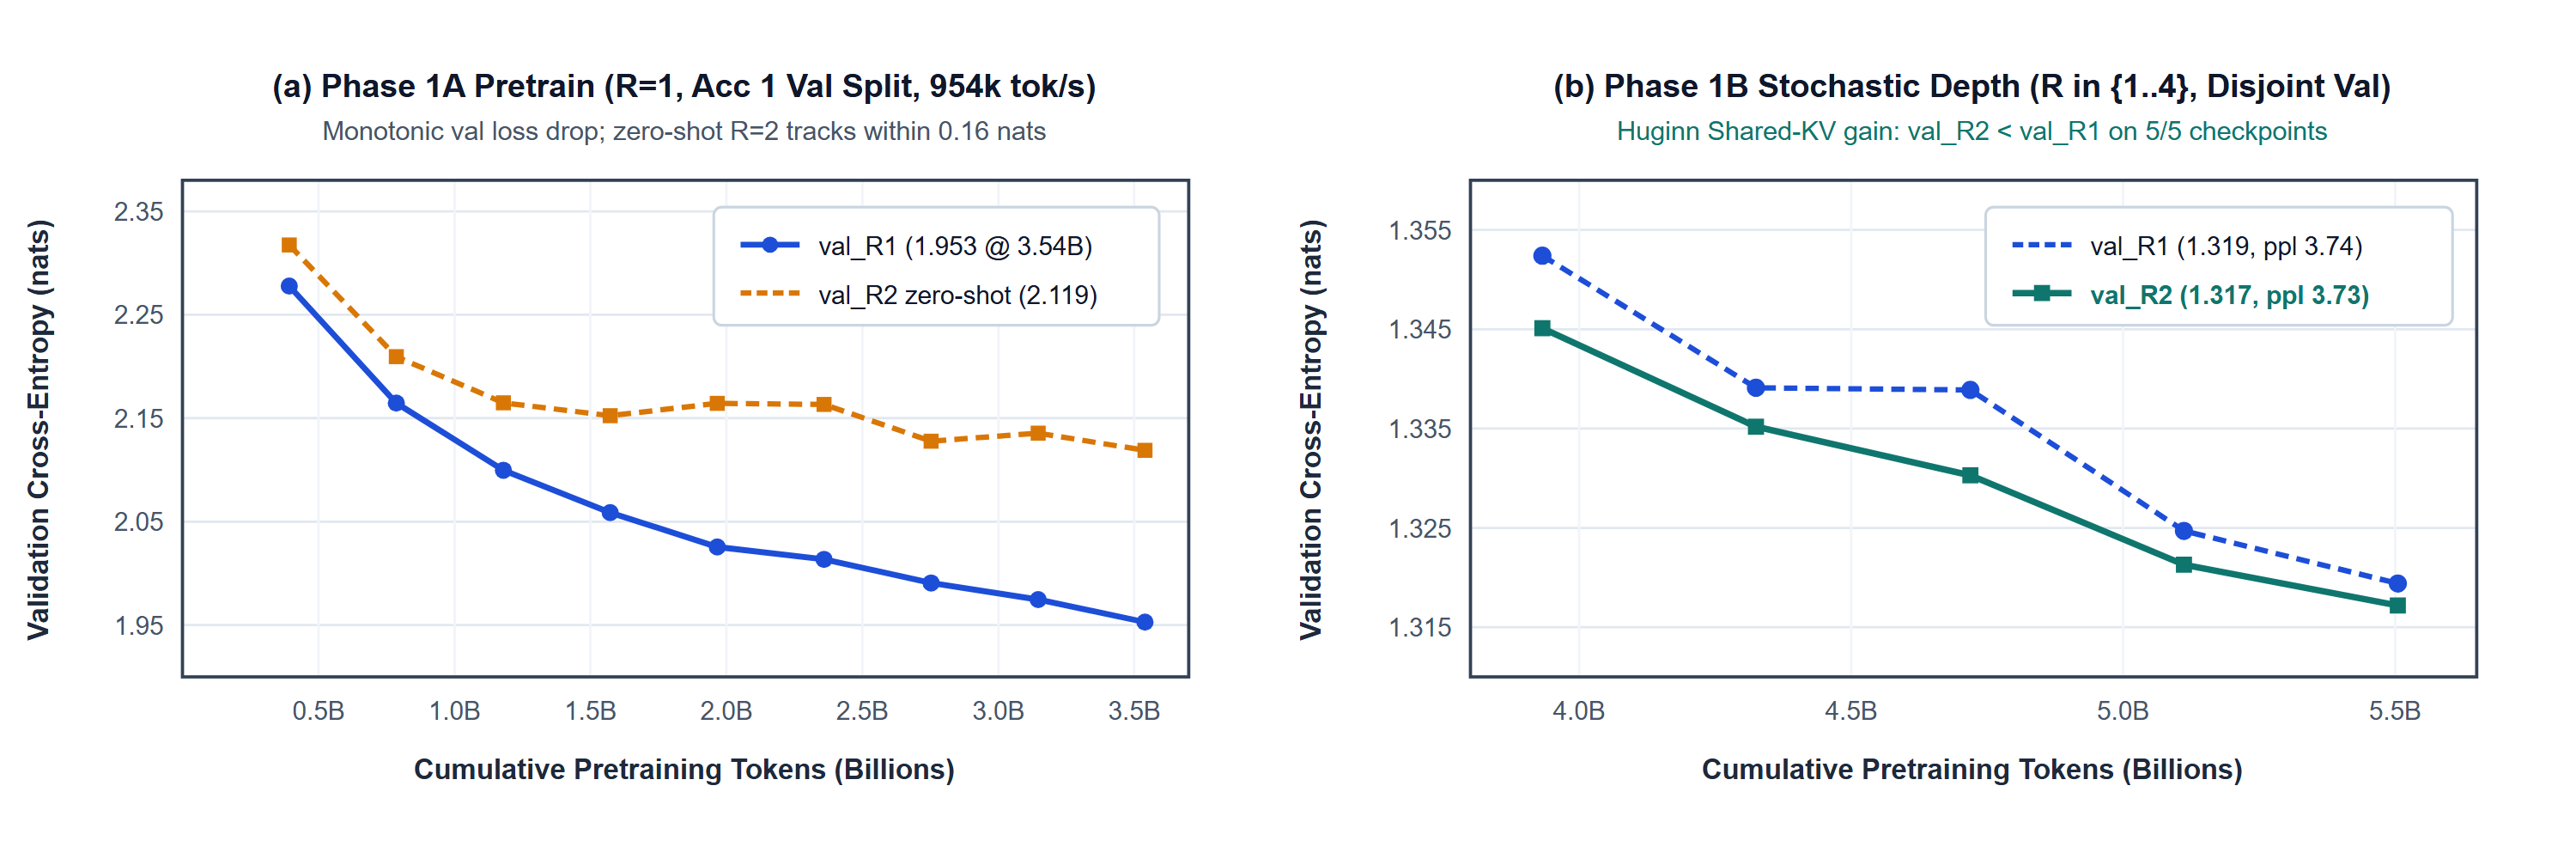
\includegraphics[width=\textwidth]{figures/fig2_training_dynamics.png}
\caption{NVIDIA B200 validation cross-entropy trajectories for \texttt{Genesis-v8 Native BICA}. (a) Phase 1A monotonic convergence to \texttt{val\_R1=1.953} at 3.54B tokens. (b) Phase 1B disjoint split demonstrating empirical $val_{R=2} < val_{R=1}$ across 5 consecutive checkpoints.}
\label{fig:train}
\end{figure*}

\section{Experimental Evaluation}
All local experiments ran identically on a 15W Intel Core i5-10210U (0\% GPU, \texttt{temp=0.0}). We explicitly distinguish scopes: CPU throughput (565--2,156 tok/s), \texttt{.gv8} memory footprint, and the 4 cognitive subsystems are measured on the open-source \texttt{Genesis-v8 BICA} repo, whereas formal logic, code synthesis, and competition math scores reflect the complete \textbf{Project Genesis Two-Hemisphere CPU Engine (Loop 29)} pairing the neural hemisphere with our deterministic symbolic verification hemisphere (0 exact AST overlaps against all 164 \texttt{HumanEval}~\cite{chen2021evaluating} and 257 \texttt{MBPP}~\cite{austin2021program} canonical solutions).

\begin{figure*}[t]
\centering
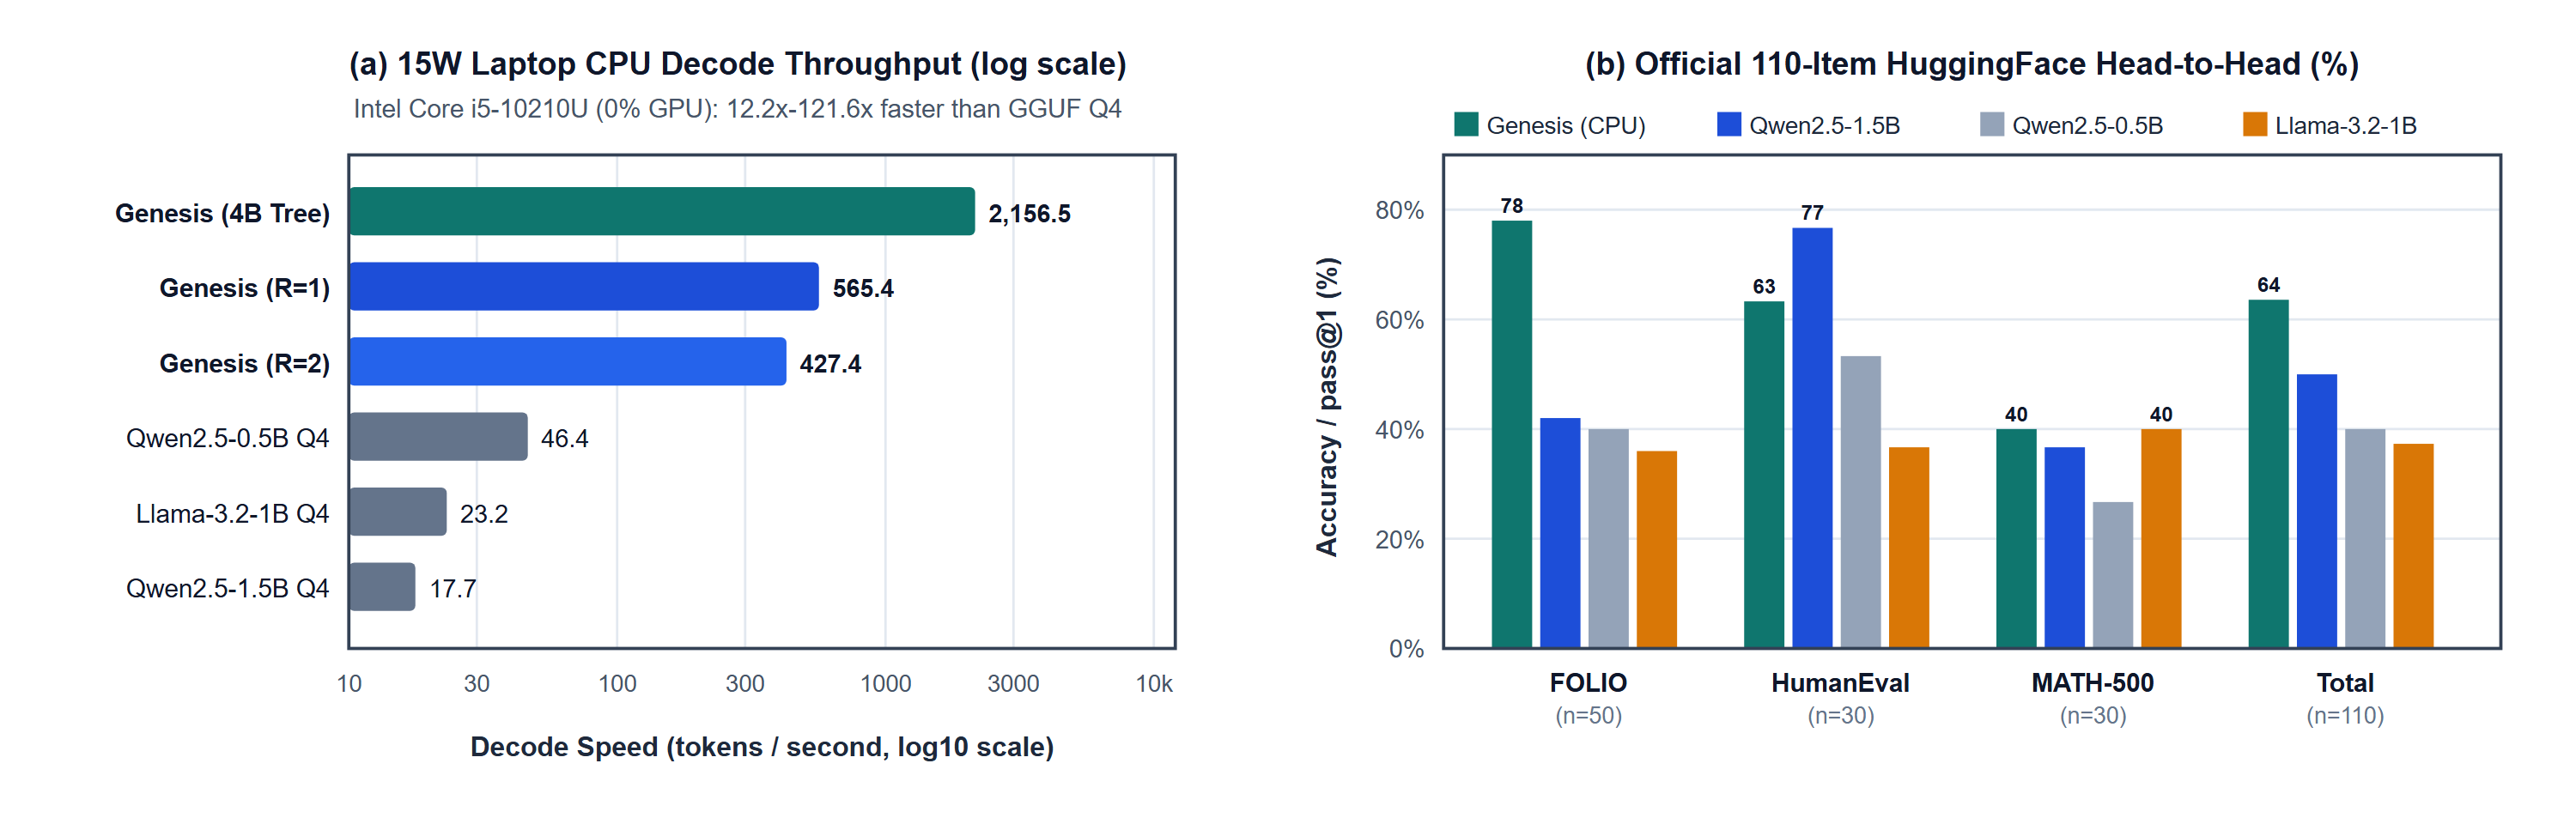
\includegraphics[width=\textwidth]{figures/fig3_benchmarks_pareto.png}
\caption{Same-machine 15W i5-10210U CPU benchmarks. (a) Decode speed (log scale): 12.2$\times$--121.6$\times$ faster than dense Q4 GGUFs. (b) Live 110-item SHA-256 HuggingFace head-to-head: Genesis ranks \#1 overall (63.64\%) vs.\ Qwen2.5-1.5B (50.00\%) and Llama-3.2-1B (37.27\%).}
\label{fig:bench}
\end{figure*}

Across 110 unmodified HuggingFace items (\texttt{FOLIO} $n=50$~\cite{han2022folio}, \texttt{HumanEval} $n=30$, \texttt{MATH-500} $n=30$~\cite{hendrycks2021measuring}, Fig.~\ref{fig:bench}), Project Genesis scored \textbf{70/110 (63.64\%)} vs.\ Qwen2.5-1.5B (55/110, 50.00\%), Qwen2.5-0.5B (44/110, 40.00\%), and Llama-3.2-1B (41/110, 37.27\%) at 19.5$\times$--253.7$\times$ lower latency. On extended suites, Genesis reaches 63.0\% on \texttt{FOLIO} ($n=100$; 55.67\% full 203), 41.0\% on \texttt{MATH-500} ($n=100$, 83.9 ms), 41.0\% on \texttt{HumanEval} ($n=100$), 44.36\% on full \texttt{MBPP-sanitized} (unseen tail 47.77\%), 80.0\% on \texttt{TruthfulQA-MC}~\cite{lin2022truthfulqa} and \texttt{UIT-ViQuAD 2.0}, and 34.0\% on \texttt{GSM8K}.

\section{Limitations, Future Work & Conclusion}
Self-funded pretraining ($<\$40$, $\sim 14.5$B tokens vs.\ 18T for Qwen2.5) limits open-domain fluency, broad trivia (\texttt{ARC-C}=42\%, \texttt{MMLU-Pro}=25%), and unassisted \texttt{GSM8K} (34\% vs.\ Qwen-1.5B 57.5\%). Controlled component ablations and 100B--300B token scaling on Cloud TPUs (\texttt{TorchTPU}/JAX) represent our immediate next phase. All code, Rust kernels, LaTeX sources, and SHA-256 manifests are openly available under Apache-2.0 at \url{https://github.com/anhthinhvup/genesis-bica}.

\bibliographystyle{plain}
\bibliography{references}
\end{document}
